\chapter{Durchführung- und Auftragsbearbeitung}
\label{cha:Durchfuehrung_und_Auftragsbearbeitung}
\input{sections/03_Einleitung}
\section{ESP8266}
	\subsection{Anschließen der Sensorik}
	Für die Aufgabe wird grundsätzlich nur ein BMP benötigt.
Da jedoch entschieden wurde, die Messdaten um Temperatur und Luftfeuchtigkeit zu erweitern, 
wird ein entsprechender zusätzlicher DHT mit eingebunden.

Da es die Sensoren für den ESP bereits auf entsprechenden Daughterboards angebracht gibt,
war es nur noch nötig diese aufzustecken. \ref{fig:dht_an_esp}
	\subsection{Sensordaten auslesen}
	Weil MicroPython auf dem ESP in Kombination mit einem MQTT-Broker schon 
zuvor im Unterricht Probleme bereitet hat, haben wir uns dazu entschieden, den ESP mit C++ zu programmieren.

Für das Handling der Sensordaten und des Timestamps, welcher später übermittelt werden soll, wurde eine separate Klasse "`sensorData"' \ref{lst:class_sensordata} angelegt.
Über den Konstruktor können die Werte an eine Klasseninstanz übergeben werden. 
Werden diese dann zum Übermitteln an den Broker benötigt, können die Werte dann einfach per Pfeiloperator ("`->"') abgefragt werden.

Für sowohl den DHT als auch den BMP wurde die "`Adafruit\_Sensor"'-Bibliothek verwendet.
Diese wird mit 
\begin{lstlisting}[language=C++]
	#include Adafruit_Sensor.h
\end{lstlisting}
eingebunden.

\subsubsection{Auslesen DHT}
	Beim DHT war es noch zusätzlich notwendig, die "`DHT"'-Bibliothek mit 
\begin{lstlisting}[language=C++]
	#include <DHT.h>
\end{lstlisting}
 	einzubinden.
	Wenn die Bibliothek eingebunden ist, kann eine Instanz vom Typ "`DHT"' und der Bezeichnung "`dht"' mit der Zeile 
\begin{lstlisting}[language=C++]
	DHT dht(02,DHT22);
\end{lstlisting}	
	erzeugt werden.
	Die "`02"' beschreibt den Pin, auf welchen der DHT die Daten sendet und das "`DHT22"' beschreibt den genauen Typ des DHT.
	
	In der Funktion \textit{void setup()} wird mit der Zeile
\begin{lstlisting}[language=C++]
	dht.begin();
\end{lstlisting}
	das Auslesen des Pins gestartet. 
	Jetzt kann in der Funktion \textit{void loop()} mit 
\begin{lstlisting}[language=C++]
	dht.readTemperature();
\end{lstlisting}
	die aktuelle Temperatur und mit
\begin{lstlisting}[language=C++]
	dht.readHumidity();
\end{lstlisting}
	die aktuelle Luftfeuchtigkeit ausgelesen werden.
	
\subsubsection{Auslesen BMP}
	Für den BMP musste noch die "`Adafruit\_BMP085"'-Bibliothek eingebunden werden.
	Hier wurde dann ebenfalls eine Klasseninstanz mit 
\begin{lstlisting}[language=C++]
	Adafruit_BMP085 bmp180;
\end{lstlisting}
	erzeugt. Beim BMP war keine weitere Konfiguration notwendig.
	
	Ähnlich zum DHT wird auch beim BMP das Auslesen mit 
\begin{lstlisting}[language=C++]
	bmp180.begin();
\end{lstlisting}
	in der \textit{void setup()} gestartet.
	Da der Luftdruck jedoch je nach Wetterlage variieren kann, muss der Sensor am Start referenziert werden.
	Da die Höhe des Klassenzimmers bekannt ist (469 m über N.N.), wird immer beim Start mit 
\begin{lstlisting}[language=C++]
	seaLevelPressure = bmp180.readSealevelPressure(currentAltitude);
\end{lstlisting}
	der aktuelle Luftdruck gemessen und auf den Luftdruck auf Meereshöhe rückgerechnet. Dieser wird dann in der Variable "`seaLevelPressure"' gespeichert, welche dann als Referenz für die weiteren Messungen verwendet wird.
	
	Da der BMP mit 
\begin{lstlisting}[language=C++]
	bmp180.readTemperature();
\end{lstlisting}
	ebenfalls die aktuelle Temperatur messen kann, wird aus den Temperaturen des DHT und BMP der Mittelwert gebildet und abgespeichert.
	Die aktuelle Höhe kann über 
\begin{lstlisting}[language=C++]
	bmp180.readAltitude(seaLevelPressure);
\end{lstlisting}
	in Anhängigkeit des zuvor referenzierten Luftdrucks gemessen werden.
	Da auch der Luftdruck auf der Website erscheinen soll, wird dieser mit 
\begin{lstlisting}[language=C++]
	(float)bmp180.readPressure()/100;
\end{lstlisting}
	ausgelesen.
	Die Konvertierung zu einem Float und das Dividieren durch 100 sorgt dafür, dass der Druck in mBar mit Nachkommastellen zurückgeliefert wird.

\subsubsection{Erzeugung Timestamp}
	Da der Timestamp keine zeitliche Abweichung zu den Messergebnissen haben soll, wird dieser annähernd zeitgleich ebenfalls durch den ESP abgespeichert.
	Aufgrund der Tatsache, dass der ESP über keine interne Uhr verfügt und auch 
\begin{lstlisting}[language=C++]
	std::chrono::system_clock::now;
\end{lstlisting}
	nur auf den NTP-Server des verbundenen WLAN-Routers zugreift, kann diese Bibliothek nicht verwendet werden. Wenn der ESP mit dem Hotspot eines Smartphones verbunden wird, liefert 
\begin{lstlisting}[language=C++]
	std::chrono::system_clock::now;
\end{lstlisting}
	nur noch "`0000000000"' zurück, da das Smartphone keinen NTP-Server zur Verfügung stellt.
	Diese Limitierung kann jedoch umgangen werden, indem direkt auf eine URL eines NTP-Servers verwiesen wird, von welchem dann die aktuelle Zeit bezogen werden kann.
	Für den direkten Verweis auf einen NTP-Server sind sowohl die "`NTPClient"' als auch die "`WiFiUdp"'-Bibliothek nötig.
	Die "`WiFiUdp"'-Instanz kann ohne weitere Parameter initialisiert werden:
\begin{lstlisting}[language=C++]
	WiFiUDP ntpUDP;
\end{lstlisting}
	Beim NTPClient müssen die WiFiUdp-Instanz, die URL des NTP-Servers und die Verschiebung zur UTC in Sekunden angegeben werden: 
\begin{lstlisting}[language=C++]
	NTPClient timeClient(ntpUDP, "pool.ntp.org", 7200);
\end{lstlisting}
	Auch der "`timeClient"' muss mit 
\begin{lstlisting}[language=C++]
	timeClient.begin();
\end{lstlisting}
	gestartet werden, jedoch ist hier naheliegenderweise eine WLAN-Verbindung notwendig.
	Bevor die Zeit abgefragt wird, muss der Client mit 
\begin{lstlisting}[language=C++]
	timeClient.update();
\end{lstlisting}
	geupdated werden, dass tatsächlich die aktuelle Zeit zurückgeliefert wird.
	Für einen Timestamp mit Uhrzeit und Datum muss zuerst die "`EpochTime"' abgefragt werden:
\begin{lstlisting}[language=C++]
	timeClient.getEpochTime();
\end{lstlisting}
	Dies liefert einen Unix-Timestamp zurück.
	Dieser kann dann mit 
\begin{lstlisting}[language=C++]
	strftime(timestamp, 20, "`\%Y-\%m-\%d \%H:\%M:\%S"' ,localtime(\&now));
\end{lstlisting}
	in ein YYYY-MM-DD HH:MM:SS Format umformatiert und in die Variable "`timestamp"' abgespeichert werden, wobei die Variable "`now"' die zuvor abgefragte "`EpochTime"' ist.
	
	\subsection{WLAN Verbindung}
	Für die WLAN-Verbindung wurde die "`ESP8266WiFi"'-Bibliothek benötigt.
Der Verbindungsvorgang wurde in eine separate Funktion ausgelagtert, welcher die SSID und das Passwort übergeben werden.\ref{lst:wificonnect}
Diese Funktion wird immer initial in der \textit{void setup()}-Funktion aufgerufen, um die WLAN-Verbindung herzustellen.
Ebenfalls wird bei jedem Durchlauf der \textit{void loop()}-Funktion mit \textit{if(WiFi.status() != WL\_CONNECTED)} überprüft, ob die WLAN-Verbindung noch besteht.
Sollte dies nicht mehr der Fall sein, so wird die Funktion zur Verbindung mit dem WLAN erneut aufgerufen.
	\subsection{Verbinden zu und publishen auf MQTT Broker}
	Um eine Verbindung zu einem (öffentlichen) MQTT-Broker herstellen zu können, wird zusätzlich zur bereits eingebundenen "`ESP8266WiFi"' auch die "`PubSubClient"'-Bibliothek benötigt.
Allerdings ist es nötig, zuerst eine Instanz der Klasse "`WiFiClient"' mit \textit{WiFiClient espClient;} zu erzeugen.
Diese Instanz wird dann wiederum bei der Instanziierung der "`PubSubClient"'-Klasse übergeben: \textit{PubSubClient client(espClient);}.
Auch die Verbindungsherstellung zum MQTT-Broker wurde in eine Funktion ausgelagert.\ref{lst:mqttconnect}
Dieser wird die URL des Brokers sowie der zugehörige Port übergeben.
Die Funktion wird ebenfalls in der \textit{void setup()}-Funktion für die initiale Verbindung aufgerufen, dieser Aufruf erfolgt nachdem die WLAN-Verbindung erfolgreich hergestellt wurde.
Auch beim MQTT-Broker wird bei jedem Durchlauf der \textit{void loop()}-Funktion mit \textit{if(!client.connected())} überprüft, ob die Verbindung noch offen ist um diese gegebenenfalls wiederherzustellen.
Bevor die Messwerte dann an den Broker gepublisht werden können, müssen diese als JSON-Objekt serialisiert werden.
Hierfür wird die "`ArduinoJson"'-Bibliothek eingebunden.
Die Klasseninstanz wird hier mit \textit{JsonDocument serializedData;} nur lokal in der \textit{void loop()}-Funktion erzeugt, sodass dieses in jedem Durchlauf neu erzeugt und am Ende wieder verworfen wird.
Die "`serializedData"'-Instanz wird nun mit den Keys und den enstprechenden Values befüllt.\ref{lst:writejson}
Da jedoch keine Instanz eines JsonDocuments an den MQTT-Broker gepublisht werden kann, muss die Zeichenanzahl bestimmt und der Inhalt zuerst wieder in ein Characterarray gespeichert werden: \textit{size\_t n = serializeJson(serializedData, buffer);}.
Nun können die Messwerte zusammen mit den Keys an den Broker gesendet werden : \textit{client.publish(topic, buffer, n)}.
Hier muss noch die Topic mit angegeben werden, welche dann später wieder vom Server abgefragt werden kann.
Zusätzlich wird der Character Array und die Länge dessen übergeben.
	
\section{Raspberry Pi}
	\subsection{Installation benötigter Software}
	Auf dem Raspberry Pi wurden enstprechend der MariaDB-Server, der NodeJS-Server sowie NPM installiert. NPM wird hier für die Installation von Paketen, welche der NodeJS-Server benötigt, verwendet.
	\subsection{Datenbank}
	\subsubsection{Datenbankplanung}
Als erstes musste ein passendes Datenbankschema entworfen werden, in dem die Sensordaten passend gespeichert werden können. Das folgende Schema stellt die Datenbankstruktur vor.
\begin{figure}[H]
	\centering
	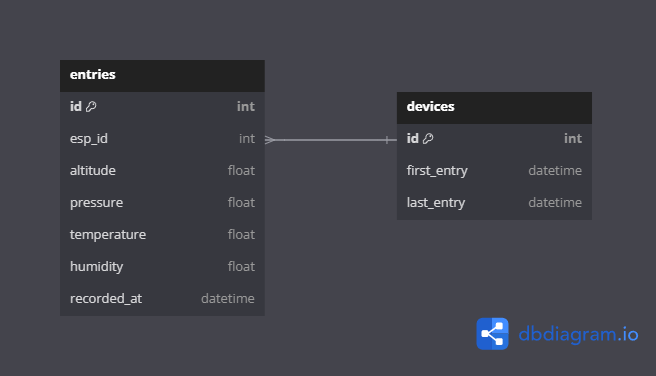
\includegraphics[width=15cm]{images/db_diagram.png}
	\caption{Datenbankdiagramm}
	\label{fig:db_diagram}
\end{figure}
Die Tabelle "`entries"' enthält die Messdaten, Höhe über N.N., den Luftdruck, die Temperatur, die Luftfeuchtigkeit und einen Zeitstempel des Messzeitpunktes, welche das Backend vom MQTT-Broker erhält. Außerdem wurde die Datenbank um eine Tabelle "`devices"' erweitert. Diese Tabelle speichert die einzigartigen Geräte, welche Daten in die Datenbank gespeichert haben. Sie enthält die "`ESP\_ID"' im Feld id, den ersten und letzten Eintrag des Geräts.

\subsubsection{Einrichtung der Datenbank}
Die MariaDB Datenbank wurde durch ein Script initialisiert.  Dieses sollte nur ein einziges mal, vor Inbetriebnahme des Systems ausgeführt werden, da durch Zeile eins, "`DROP DATABASE esp\_data;"', die Datenbank und alle in ihr enthaltenen Daten gelöscht werden. 
\begin{figure}[H]
	\centering
	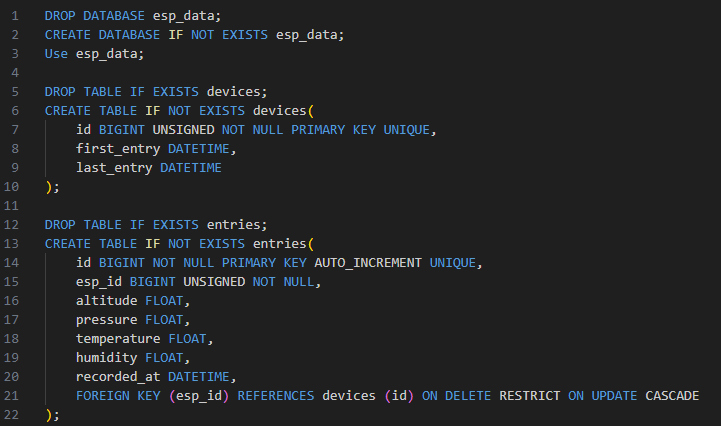
\includegraphics[width=15cm]{images/db_initialisation_script.png}
	\caption{Datenbankinitialisierungsscript}
	\label{fig:db_initialisation_script}
\end{figure}
	\subsection{Programmierung des NodeJS-Servers}
	\subsubsection{Konfiguration der MariaDB Verbindung}
Das folgende Code Snippet bescheibt die Datenbankverbindung zum lokal installierten Datenbankserver. Es enthält die benötigten Bibliotheken, den Userzugang und die Datenbank auf dem Server mit dem sich der Webserver verbindet.
\begin{lstlisting}[language=java]
	//MariaDB
	const mariadb = require('mariadb');
	const pool = mariadb.createPool({
		host: 'localhost',
		user: 'root',
		password: 'toor',
		database: 'esp_data',
		connectionLimit: 2
	});
\end{lstlisting}

\subsubsection{Konfiguration der MQTT Verbindung}
Der folgende Code bescheibt die Konfiguration des MQTT Objekts. Hier wurde nicht, wie geplant, mit HiveMQ gearbeitet, sondern mit Mosquitto. Getestet wurde auch der Eclipseprojects MQTT Broker. Für unser Projekt war aber Mosquitto der stabilste öffentliche Broker. Auch hier werden erst die benötigten Bibliotheken angegeben. Es folgen die Broker-URL, der Port und das Topic. Dann wird eine Verbindung aufgebaut und sich als Abonnent am Topic angemeldet, so dass der Broker Updates an den Webserver schicken kann.
\begin{lstlisting}[language=java]
	//MQTT
	const mqtt = require('mqtt');
	const { each, error, ready } = require("jquery");
	const protocol = 'mqtt';
	const mqtt_broker = 'test.mosquitto.org';
	//const mqtt_broker = 'mqtt.eclipseprojects.io';
	const mqtt_port = 1883;
	const mqtt_url = protocol + '://' + mqtt_broker + ':' + mqtt_port;
	const mqtt_topic = 'est/katastrophenprojekt/espdaten';
	const mqtt_client = mqtt.connect(mqtt_url, keepalive = 60);
	let topic = mqtt_client.subscribe(mqtt_topic);
\end{lstlisting}

\subsubsection{Event: MQTT Message}
Dieses Event beschreibt was passiert, wenn eine Nachricht vom MQTT-Broker empfangen wird. Erst wird die Nachricht in die Konsole geschrieben, was beim Debugging hilft und dann wird die Nachricht in der Funktion: messageRecieved weiterverarbeitet.
\begin{lstlisting}[language=java]
	mqtt_client.on('message', (topic, message) => {
		console.log('Message:' + message);
		messageRecieved(message);
		//console.log('success');
	});
\end{lstlisting}

\subsubsection{Funktion: messageRecieved}
In der Funktion messageRecieved(message) wird, wie oben erwähnt, die Nachricht verarbeitet. Da die Daten in zwei verschiedene Tabellen in der Datenbank geschrieben werden müssen werden hier auch zwei SQL-Queries ausgeführt. 
\begin{lstlisting}[language=java]
	async function messageRecieved(message) {
		let conn;
		let jsonObj = JSON.parse(message);
		try {
			conn = await pool.getConnection();
			const res = await conn.query("INSERT INTO devices (id, first_entry, last_entry) VALUES (?, ?, ?) ON DUPLICATE KEY UPDATE last_entry = VALUES (last_entry);", [jsonObj.device_id, jsonObj.timestamp, jsonObj.timestamp]);
			console.log(res);
			const entry = await conn.query("INSERT INTO esp_data.entries (esp_id, altitude, pressure, temperature, humidity, recorded_at) VALUES (?, ?, ?, ?, ?, ?);", [jsonObj.device_id, jsonObj.altitude, jsonObj.airPressure, jsonObj.temperature, jsonObj.humidity, jsonObj.timestamp]);
			console.log(entry);
		} catch(err) {
			console.log("Error: " + err);
			throw err;
		}
		finally {
			if(conn) return conn.end();
		}
	}
\end{lstlisting}

\subsubsection{Route: getData}
Diese Route wird aufgerufen, wenn die Route: Index geladen wird. Dabei wird die asynchrone Funktion readData(req, res) ausgeführt.
\begin{lstlisting}[language=java]
	app.get("/data", (req, res) => {
		readData(req, res);
	});
\end{lstlisting}

\subsubsection{Funktion: readData}
Die Funktion readData(req, res) liest Daten aus der Datenbank und sendet diese and die Website, damit sie dort visualisiert werden können.
\begin{lstlisting}[language=java]
	async function readData(req, res) {
		let conn;
		try {
			conn = await pool.getConnection();
			data = await conn.query("SELECT * FROM (SELECT * FROM entries ORDER BY recorded_at DESC LIMIT 1000) AS subquery ORDER BY id ASC;");
			res.json(data);
		} catch (err) {
			throw err;
		} finally {
			if (conn) conn.end();
		}
	}
\end{lstlisting}
	\subsection{Programierung der Website zur Datenvisualisierung}
	Bei der Website wurde Chart.js für die grafische Darstellung der Messwerte benutzt.
Die Messwerte wurden mithilfe der "`fetch"'-API vom Backend angefragt und dann dem zugehörigen Diagramm zugeordnet.
Auf der Website wurden dann vier Diagramme für die Temperatur, Luftfeuchtigkeit, Höhe über N.N. und den Luftdruck angezeigt. \ref{fig:website}
Die Daten werden alle fünf Sekunden neu abgefragt und entsprechend aktualisiert.
	
\section{Knackpunkte, Abweichungen, Anpassungen, Entscheidungen}
	\subsection{Knackpunkte}
	Die Knackpunkte im Projekt sind vorwiegend durch kleinere, jedoch schwer zu lokalisierende Fehler entstanden. \newline

Bei der Datenbank gab es initiale Schwierigkeiten mit dem Initialisierungsskript, welches das Setup und vorwiegend mehrfache Setups stark vereinfacht und beschleunigt.
Letztendlich ließen sich hier die Schwierigkeiten auf inkorrekte Syntax zurückführen, welche jedoch teilweise sehr schwer zu lokalisieren war. \newline
Auch bei der Schnittstelle zwischen der Datenbank und dem NodeJS-Backend gab es aufgrund von Syntaxfehlern mittlere Verzögerungen.
Letztendlich waren wir jedoch in der Lage, alle Fehler zu beheben. \newline
Beim ESP gab es ebenfalls kleinere Startschwierigkeiten, die Verbindung zum Broker konnte anfangs nicht hergestellt werden, was dann jedoch auf einen inkorrekten Port und eine fehlerhafte Klasseninstanziierung zurückzuführen war.
Da der ESP keine interne Zeit hat und seine Zeit immer von einem NTP-Server bezieht gab es auch hier kleinere Umstände.
Da der Hotspot eines Smartphones keinen NTP-Server direkt bereitstellt, musste das Auslesen der Zeit umprogrammiert werden, sodass nicht nur leere Timestamps zurückgeliefert wurden.
	\subsection{Abweichungen}
	Trotz der zuvor erwähnten Komplikationen waren wir in der Lage das Projekt in vollem Umfang noch rechtzeitig fertigzustellen.
Die Einzige Abweichung war der MQTT-Broker. Da HiveMQ nicht stabil zur verfügung stand, wurde ein anderer öffentlicher Broker, Mosquitto, verwendet.
	\subsection{Anpassungen}
	Da wir ausreichend Zeit für etwaige Schwierigkeiten mit eingeplant hatten, mussten keine Anpassungen am finalen Produkt vorgenommen werden.
	\subsection{Entscheidungen}
	Entsprechend der Tatsache, dass es weder Abweichungen noch Anpassungen an der Projektplanung gab, war es nicht vonnöten, Entscheidungen bezüglich möglichen Anpassungen zu treffen.
\section{Qualitätssicherung}
	\input{sections/06_Qualitaetssicherung/qualiteatssicherung}
	